\addcontentsline{toc}{subsection}{Plane Curves and Parametric Equations}
\subsection*{Plane Curves and Parametric Equations}

Until now, you have been representing a graph by a single equation involving two variables. Now, we will introduce a third variable to describe some curve in the plane.

\begin{tcolorbox}[title= DEFINITIONS OF A PLANE CURVE,colframe=black,sharp corners,colback=white,colbacktitle=white,coltitle=black]

    If $f$ and $g$ are continuous functions of $t$ on the interval $I$, then the equations $x=f(t)$ and $y=g(t)$ are called \textbf{parametric equations} and $t$ is called the \textbf{parameter}. Together, the parametric equations produce the graph called a \textbf{plane curve}.

\end{tcolorbox}
\vspace{.1cm}
Try sketching the plane curve given by the parametric equations $x=t^2-4$ and $\displaystyle y=\frac{t}{2}$ for $-2\le t\le3$.

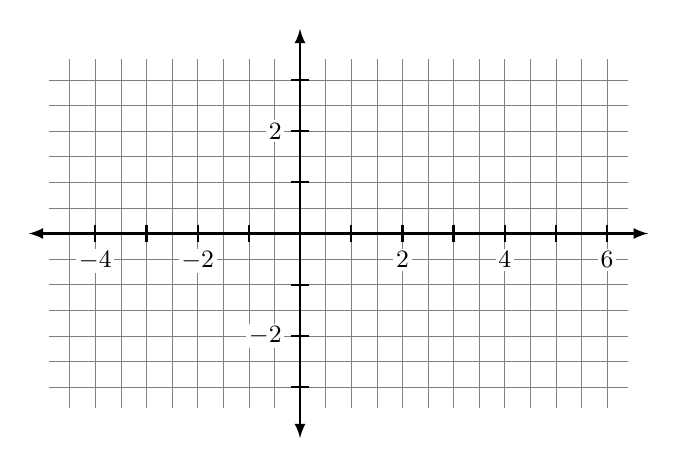
\begin{tikzpicture}[xscale=.65,yscale=.65]
    \draw[step=.5,style=help lines,] (-4.9,-3.4) grid (6.4,3.4);
    \draw[latex-latex, thick] (-5.3,0)--(6.8,0);
    \draw[latex-latex, thick] (0,-4)--(0,4);
    \foreach \x in {-4,-2,2,4,6}
        \draw[thick] (\x,5pt) -- (\x,-5pt) node [below=.7mm,fill=white,inner sep=1pt] {\small$\x$};
    \foreach \y in {-2,2}
        \draw[thick] (5pt,\y) -- (-5pt,\y) node [left=.7mm,fill=white,inner sep=1pt] {\small$\y$};
    \foreach \x in {-3,-1,1,3,5}
        \draw[thick] (\x,5pt) -- (\x,-5pt);
    \foreach \y in {-3,3,-1,1}
        \draw[thick] (5pt,\y) -- (-5pt,\y);
\end{tikzpicture}

Now, eliminate the parameter to find the Cartesian equation of the curve.
\vspace{2cm}

Sketch the curve represented by $x=3\cos\theta$ and $y=4\sin\theta$, $0\le\theta\le2\pi$. Then, eliminate the parameter.

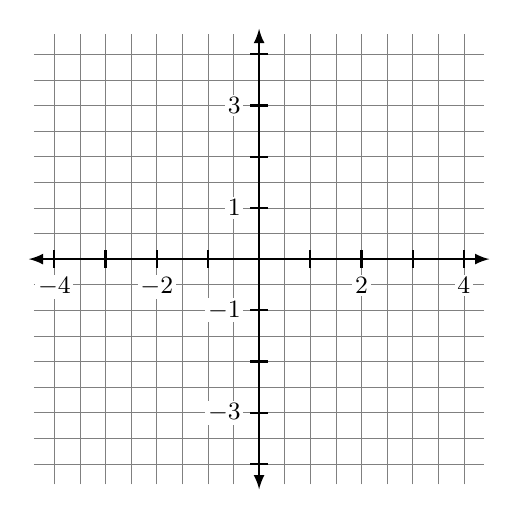
\begin{tikzpicture}[xscale=.65,yscale=.65]
    \draw[step=.5,style=help lines,] (-4.4,-4.4) grid (4.4,4.4);
    \draw[latex-latex, thick] (-4.5,0)--(4.5,0);
    \draw[latex-latex, thick] (0,-4.5)--(0,4.5);
    \foreach \x in {-4,-2,2,4}
        \draw[thick] (\x,5pt) -- (\x,-5pt) node [below=.7mm,fill=white,inner sep=1pt] {\small$\x$};
    \foreach \y in {-1,1,-3,3}
        \draw[thick] (5pt,\y) -- (-5pt,\y) node [left=.7mm,fill=white,inner sep=1pt] {\small$\y$};
    \foreach \x in {-3,-1,1,3}
        \draw[thick] (\x,5pt) -- (\x,-5pt);
    \foreach \y in {-2,2,-4,4}
        \draw[thick] (5pt,\y) -- (-5pt,\y);
\end{tikzpicture}




\newpage
